\documentclass[17pt, a0paper, portrait, margin=0mm, innermargin=15mm,
     blockverticalspace=15mm, colspace=15mm, subcolspace=8mm]{tikzposter} %Options for format can be included here


 % Title, Author, Institute
\title{Erasing watermarks on images using blind sources separation}
\author{}
\institute{\textsc{BATY L\'eo, BRUNOD-INDRIOGO Luca, EDDINE NAJJAR Chiheb, LAURET J\'er\'emy}}
%\titlegraphic{\includegraphics[height = 5cm]{ENPC.pdf}}
 %Choose Layout
%\usetheme{Envelope} % Default, Rays, Basic, Simple, Envelope, Wave, Board, Autum, Desert


\definecolor{mygray}{HTML}{CCCCCC} 
\definecolor{mypurple}{rgb}{0.63, 0.36, 0.94}
\definecolor{myyellow}{rgb}{1.0, 0.85, 0.0}
\definecolor{myorange}{rgb}{1.0, 0.65, 0.0}

\definecolorstyle{myColorStyle}{
	\colorlet{colorOne}{black} 
	\colorlet{colorTwo}{mygray} 
	\colorlet{colorThree}{mygray}
	\colorlet{mybackground}{mypurple!40!black}
}{
% Background Colors 
\colorlet{backgroundcolor}{mybackground!50}
\colorlet{framecolor}{black}
% Title Colors
\colorlet{titlefgcolor}{white}
\colorlet{titlebgcolor}{mypurple}
% Block Colors 
\colorlet{blocktitlebgcolor}{myorange}%colorTwo!70} 
\colorlet{blocktitlefgcolor}{black}
\colorlet{blockbodybgcolor}{mypurple!15} 
\colorlet{blockbodyfgcolor}{black}
% Innerblock Colors 
\colorlet{innerblocktitlebgcolor}{white} 
\colorlet{innerblocktitlefgcolor}{black} 
\colorlet{innerblockbodybgcolor}{white} 
\colorlet{innerblockbodyfgcolor}{black} 
% Note colors 
\colorlet{notefgcolor}{black} 
\colorlet{notebgcolor}{white} 
\colorlet{notefrcolor}{white}
}
\usecolorstyle{myColorStyle}
\usetitlestyle{VerticalShading}
\useblockstyle{Slide}
\usebackgroundstyle{Default}


\usepackage{color}
\usepackage{multicol}
\usepackage{amsmath,amssymb}
\tikzposterlatexaffectionproofoff


\let\thempfootnote\thefootnote%http://tex.stackexchange.com/questions/956/footnotemark-and-footnotetext-in-minipage#959
\newcommand\printfootnote[1]{% to get different numbers for different footnotes
\addtocounter{footnote}{1}%
\footnotetext{#1}}

\begin{document}

% Title block with title, author, logo, etc.
\maketitle

%%%%%%%%%%%%%%%%%%%%%% I - THEORY %%%%%%%%%%%%%%%%%%%%%%

%[titleleft, titleoffsetx=2em, titleoffsety=1em, bodyoffsetx=2em, bodyoffsety=1em, titlewidthscale=.6, bodywidthscale=.8, roundedcorners=14, linewidth=8mm, bodyinnersep=4em, titleinnersep=2em]

\block[]{Introduction}{



\begin{multicols}{2}

\bigskip
 
\bigskip

A watermark is a digitally added text used to copyright an image and prevent it from unrightful copy or misappropriation (cf. fig.1). This project aims at the complete removal of such watermarks.\\

We chose to use theoretical results on blind source separation in order to create an efficient watermark-erasing program.\\
We first considered the simplest case of linear watermarks, and then more realistic ones which were not necessarily linear. In each case, we assumed that we had a set of three images composed of a target image with a watermark to erase and two copies of another image, one with the same watermark and the other without any. 

\columnbreak

\begin{tikzfigure}[Examples of watermarked images\footnotemark{}]
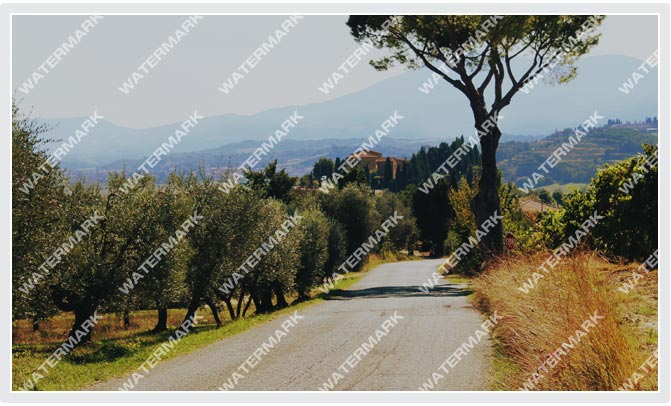
\includegraphics[width=0.15\textwidth]{img/watermarkExample1.jpg}

\includegraphics[width=0.15\textwidth]{img/watermarkExample2.jpg}
\end{tikzfigure} 

\end{multicols}
\setlength{\columnseprule}{10pt}
\def\columnseprulecolor{\color{black}}

%\begin{tikzfigure}[h]
%\begin{center}
%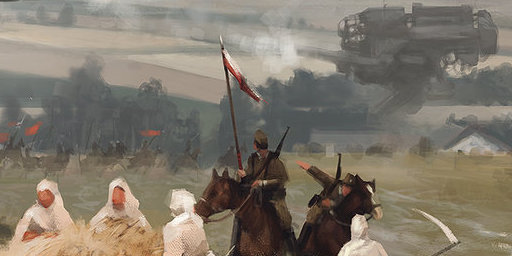
\includegraphics[width = 10cm]{image1.jpg}
%\caption{default}
%\label{default}
%\end{center}
%\end{tikzfigure}


}

\block{I - Theory and Mathematical tools}{

The observed information, contained in a random vector $\vec{x}$, is the image of an unknown random vector $\vec{s}$ by an unknown linear transformation $A$, i.e. $\vec{x} = A\vec{s}$. The question is, can we find $\vec{s}$ using only $\vec{x}$ ?
}

\begin{columns}
\column{0.5}
\block{}{
According to \textsc{Comon}'s therom, if the problem satisfies the following conditions :

\begin{itemize}
\item the components of $\vec{s}$ are independent
\item at most, one of $\vec{s}$ components is gaussian
\item $A$ is a time independant invertible matrix
\end{itemize}

then, any matrix $B$ such that the vector $B\vec{x}$ has independent components satisfies that $B\vec{x} \simeq \vec{s}$, meaning that $B\vec{x}$ is the image of $\vec{s}$ under a permutation and a homothety.

To characterize the independence of the components of a vector, we can use the
\textbf{Mutual penalized Information $J$ : }
\begin{equation}
J \left(\vec{y}\right) = \int_{\vec{t}} p_{\vec{y}} \left(\vec{t}\right) \ln \left(  \frac{p_{\vec{y}} \left(\vec{t}\right)}{\Pi_i p_{y_i}(t_i)} \right) \mathrm{d} \vec{t} + \lambda \sum_i \left( \mathrm{Var}(y_i) - 1 \right)^2 
\end{equation}
where $\vec{y} = (y_i)_i$ is a random vector, and $\lambda$ is the penalty setting.\\

}

\column{0.5}
\block{}{

$J$ satisfies the following properties :
\begin{itemize}
\item $J \geq 0$
\item $J \left(\vec{y}\right) = 0 \Leftrightarrow \vec{y}$ has independent components, and $\mathrm{Var}(y_i) = 1 ~ \forall~ i$
\end{itemize}

Now we can reformulate the problem as follows : find $B$ such that  $J( B\vec{x} ) = 0$ which is equivalent to find $\min_B J(B\vec{x})$.\\

$J$ does not only help us find a vector with independent components from $\vec{x}$ but also a bounded one.\\

To minimize $J$ over $B$ we use the gradient descent algorithm : $B_{n+1} = B_n - \mu \frac{\partial J}{\partial B}(B_n)$, where $\mu$ is the step parameter. \\

Finally, we chose to impose $\mathbb{E}[y_i] = 0$ at all times in our algorithm for mathematical simplicity.

}

\end{columns}

%%%%%%%%%%%%%%%%%%%%%% II - LINEAR WATERMARKS %%%%%%%%%%%%%%%%%%%%%%

\block{II - Case of a linear watermark}{


\begin{multicols}{2}

\begin{center}
At first, we used our algorithm\footnotemark{} in a case that matched the theoretical framework, that is to say a watermark obtained by linear combination of a text on plain background with the original image :

\begin{tikzfigure}[Input of two images with a linear watermark and one without]
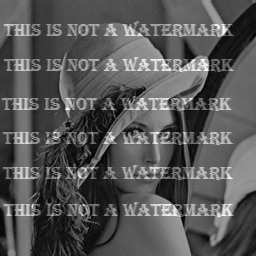
\includegraphics[width=0.1\textwidth]{img/test1.png}
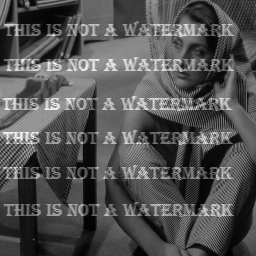
\includegraphics[width=0.1\textwidth]{img/test.png}
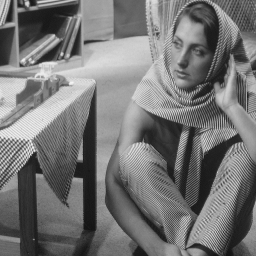
\includegraphics[width=0.1\textwidth]{img/barbara.png}
\end{tikzfigure}
\end{center} 


\columnbreak

\begin{center}
As expected, the algorithm returns both original images along with the image of the watermark:

\begin{tikzfigure}[Output of the program after 5000 iterations and $\mu=0.01$]
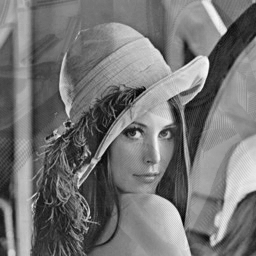
\includegraphics[width=0.1\textwidth]{img/resu1.png}

\includegraphics[width=0.1\textwidth]{img/resu2.png}
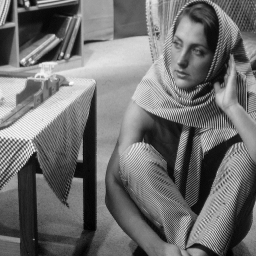
\includegraphics[width=0.1\textwidth]{img/resu3.png}
\end{tikzfigure}
\end{center} 

\end{multicols}



}

% \begin{columns}
%
% % FIRST column
%\column{0.6}% Width set relative to text width
%\block{Large Column}{Text\\Text\\Text Text Text}
%\note{Note with default behavior}
%\note[targetoffsetx=12cm, targetoffsety=-1cm, angle=20, rotate=25]
%{Note \\ offset and rotated}
% % First column - second block
%\block{Block titles with enough text will automatically obey spacing requirements }
%{Text\\Text}
% % First column - third block
%\block{Sample Block 4}{T\\E\\S\\T}
%
% % SECOND column
%\column{0.4}
% %Second column with first block’s top edge aligned with with previous column’s top.
% % Second column - first block
%\block[titleleft]{Smaller Column}{Test}
% % Second column - second block
%\block[titlewidthscale=0.6, bodywidthscale=0.8]
%{Variable width title}{Block with smaller width.}
% % Second column - third block
%\block{}{Block with no title}
% % Second column - A collection of blocks in subcolumn environment.
%\begin{subcolumns}
%    \subcolumn{0.27} \block{1}{First block.} \block{2}{Second block}
%    \subcolumn{0.4} \block{Sub-columns}{Sample subblocks\\Second subcolumn}
%    \subcolumn{0.33} \block{4}{Fourth} \block{}{Final Subcolumn block}
%\end{subcolumns}
% % Bottomblock
%\block{Final Block in column}{
%    Sample block.
%}
%\end{columns}
%\block[titleleft, titleoffsetx=2em, titleoffsety=1em, bodyoffsetx=2em,%
% bodyoffsety=-2cm, roundedcorners=10, linewidth=0mm, titlewidthscale=0.7,%
% bodywidthscale=0.9, bodyverticalshift=2cm, titleright]
%{Block outside of Columns}{Along with several options enabled}

%%%%%%%%%%%%%%%%%%%%%% III - NON-LINEAR WATERMARKS %%%%%%%%%%%%%%%%%%%%%%

\block{III - Case of a common (non-linear) watermark}{
We generalized the code to colored images working separately on each of the three RGB colors.
The case of a linear watermark is very specific and most of the commonly used watermarks are not that simple. This is why we also tried to remove a watermark made by a specialized website\footnotemark{}.


\begin{tikzfigure}[Input of two images with a non-linear watermark and one without]
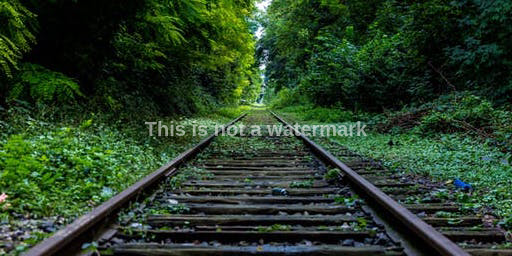
\includegraphics[width=0.2\textwidth]{img/watermarked_rails.png}
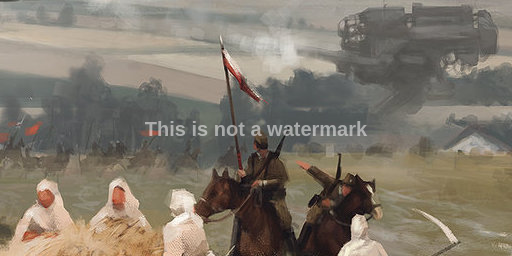
\includegraphics[width=0.2\textwidth]{img/watermarked_warscene.png}
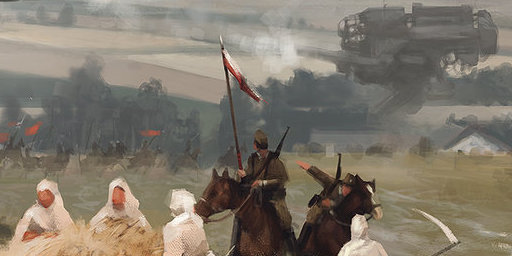
\includegraphics[width=0.2\textwidth]{img/warscene.jpg}
\end{tikzfigure} 
}

\block{}{
As the modification of the images we obtained that way were not necessarily linear, we couldn't expect to erase the watermark only by using blind source separation. The returned values are nevertheless interesting.

\begin{tikzfigure}[Result of the program]
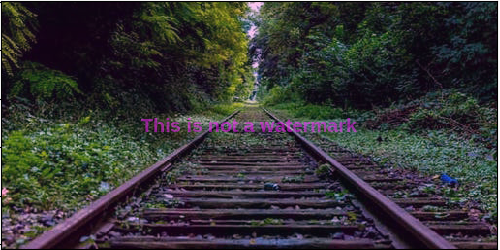
\includegraphics[width=0.2\textwidth]{img/recomposed_rails.png}

\includegraphics[width=0.2\textwidth]{img/recomposed_warscene_1.png}
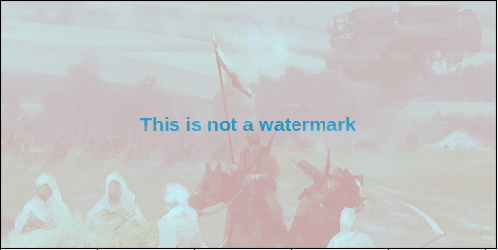
\includegraphics[width=0.2\textwidth]{img/recomposed_warscene_2.png}
\end{tikzfigure} 

The watermark barely changed and is still visible. However, the algorithm manages to isolate the letters of the watermark on a plain background.



\begin{multicols}{2}



Thus, it becomes rather easy to identify the pixels of the images that correspond to the letters. This allows to determine the kind of transformation which was applied by comparing the pixels of the image we possess with and without a watermark. Obviously, an important drawback of this method is that it is not systematic and is possibly inconclusive when the transformation is too complicated. The results were very satisfying in our case where transformations turned out to be affine.\\

\bigskip

Linear watermarking can easily be dealt with using blind source separation, but more complex and common watermarks with non-linear transformations need a complementary treatment to obtain satisfying results. What needs to be kept in mind is that the application fields of the blind source separation method are numerous and do not stop at image processing - cryptography or sound treatment for instance can also benefit from it.

\columnbreak

\begin{tikzfigure}[Final result]
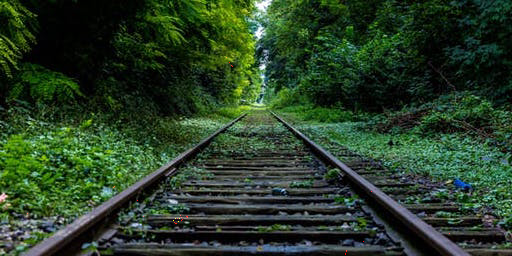
\includegraphics[width=0.2\textwidth]{img/resfinal.png}
\end{tikzfigure} 

\end{multicols}


}

%\node [above right,
%       outer sep=0pt,
%       minimum width=\paperwidth-2*\pgflinewidth,
%       minimum height=7cm,
%       align=center,font=\Huge,
%       draw,fill=blue!30,
%       ultra thick] at ([shift={(0.5*\pgflinewidth,0.5*\pgflinewidth)}]bottomleft) {Some text at the bottom};
%\end{document}


% add the footnotes in a node
\node [text width=34cm, above right] at (bottomleft) {% the bottomleft coordinate is defined by the class
\setcounter{footnote}{0}%
\printfootnote{https://www.uconomix.com/products/umark/images/watermark-tilling.jpg and https://shuttermuse.com/photologo-review-photography-logo-watermark/}
\printfootnote{https://www.umarkonline.com/}
\printfootnote{Our Python code : https://github.com/JeremyLauret/watermark-remover}

};


\node [text width=38cm, above left,font=\footnotesize,outer sep=2cm] at (bottomleft -| topright) {
\textbf{Bibliography:}\\
- M. El Rhabi, G. Gelle, H. Fenniri et G. Delaunay. "A penalized mutual information criterion for blind separation of convolutive mixtures". Signal Processing 83 (2004), 1979-1984.\\
- Massoud Babaie-Zadeh, "On Blind Source Separation in Convolutive and Non-Linear mixtures", 20 September 2002.\\
- Comon, Pierre. "Independent component analysis, a new concept?." Signal processing 36.3 (1994): 287-314.
};


\end{document}